\title{\textbf{JambaInfo: Information-Bottlenecked Jamba Architecture with Concept-Compressed SSM}}

\author{Anonymous authors}


\section{Introduction}

\subsection{Motivation}

Hybrid attention-SSM architectures have emerged as a promising direction for 
efficient transformers (Lieber et al., 2024; Dong et al., 2024). They 
combine:

\begin{itemize}
\item \textbf{Attention} for precise, content-based retrieval.
\item \textbf{State space models} for linear-time long-range mixing.

\end{itemize}
A common design choice in these architectures is to share the same input 
between the two branches: the SSM consumes the full hidden state 
$x \in \mathbb{R}^d$, just like the attention branch.

\textbf{But this is information-theoretically wasteful.} The SSM's recurrent 
state has fixed dimension, and its ability to encode information is bounded. 
Feeding it a $d$-dimensional input with high redundancy does not increase 
its effective capacity -- it just adds noise and parameters.

\subsection{The Information Bottleneck Perspective}

The Information Bottleneck (IB) principle (Tishby et al., 1999) formalizes 
the idea that a good representation $Z$ of an input $X$ for a task $Y$ 
should:

\begin{enumerate}
\item \textbf{Preserve} information about $Y$: $\max I(Z; Y)$
\item \textbf{Compress} information about $X$: $\min I(Z; X)$

\end{enumerate}
For an SSM branch, the "task" is long-range context modeling. A bottleneck 
$Z = f(X)$ with $|Z| < |X|$ forces the SSM to encode only the essential 
concepts, discarding redundancy.

\subsection{Problem Statement}

Given an input $X \in \mathbb{R}^{B \times L \times d}$ and a hybrid block 
with an SSM branch, we ask: **should the SSM see the full $X$ or a 
compressed version?**

We hypothesize that the compressed version is better, and formalize this as:

\[
\text{SSM}_\text{concept}(X) = \text{SSM}\!\left(W_\text{up} \cdot \text{GELU}(W_\text{down} X)\right)
\tag{1.1}
\]

with $W_\text{down} \in \mathbb{R}^{b \times d}$, $b \ll d$.

\subsection{Our Approach: JambaInfo}

JambaInfo combines three ideas:

\subsubsection{Differential Attention Branch}

Two Q-K pairs, ReLU-damped subtraction (Ye et al., 2024):

\[
A_\text{diff} = \text{ReLU}(A_1 - 0.2 A_2)
\tag{1.2}
\]

\subsubsection{Concept-Bottlenecked SSM Branch}

The SSM input is compressed through a low-rank concept bottleneck:

\[
z = W_\text{up} \cdot \text{GELU}(W_\text{down} x)
\tag{1.3}
\]

with $b = 256$.

\subsubsection{Learned Fusion}

\[
\text{out} = (1 - \alpha) \odot A_\text{diff} + \alpha \odot M_\text{concept}
\tag{1.4}
\]

with $\alpha = \sigma(w)$ and $w_0 = -2$ (favoring attention initially).

\subsection{Contributions}

\begin{itemize}
\item \textbf{An Information-Bottlenecked SSM branch.} We introduce a concept
  bottleneck between the hidden state and the SSM, motivated by IB theory.
\item \textbf{Dual operational modes.} JambaInfo supports a "retrieval" mode (default)
  and a "compression" mode, configurable per layer.
\item \textbf{A production-hardened implementation.} We handle four architectures,
  with strict weight-transfer validation.
\item \textbf{An honest evaluation.} We report the accuracy, parameter cost, and
  bottleneck-dimension sensitivity.
\item \textbf{Full reproducibility.} Code, weights, and scripts released.

\end{itemize}
\subsection{Paper Organization}

Section 2 reviews related work. Section 3 provides background on IB, 
attention, and SSMs. Section 4 presents JambaInfo. Section 5 describes 
integration. Section 6 details the setup. Section 7 reports results. 
Section 8 analyzes the bottleneck. Section 9 discusses guidance. Section 10 
lists limitations. Section 11 concludes.



\subsection{Notation}

\begin{lstlisting}

---
\end{lstlisting}

\section{Related Work}

\subsection{Information Bottleneck}

\textbf{Tishby et al. (1999)} introduced the Information Bottleneck principle 
for representation learning. \textbf{Alemi et al. (2017)} formulated the VIB 
(Variational IB) for deep networks. \textbf{Shwartz-Ziv \& Tishby (2017)} 
analyzed IB in training dynamics.

Our work is the first (to our knowledge) to apply IB explicitly to the SSM 
branch of a hybrid architecture.

\subsection{Hybrid Attention-SSM}

\textbf{Jamba} (Lieber et al., 2024) interleaves transformer and Mamba layers. 
\textbf{Zamba} (Glorioso et al., 2024) shares attention blocks. \textbf{Hymba} (Dong 
et al., 2024) fuses attention and SSM in a single block. \textbf{Samba} (Ren et 
al., 2024) uses a similar design.

\textbf{Our distinction.} We add an \textbf{explicit bottleneck} between the input 
and the SSM branch, forcing the SSM to operate on compressed concepts.

\subsection{Differential Attention}

\textbf{Differential Transformer} (Ye et al., 2024) introduces two-Q-K 
subtraction for noise reduction. We use this as our attention branch with 
a softened damping ($\lambda = 0.2$ vs Ye's $0.8$).

\subsection{State Space Models}

\textbf{S4} (Gu et al., 2021), \textbf{Mamba} (Gu \& Dao, 2023), \textbf{HGRN-2} (Qin et 
al., 2024) are linear-time recurrent models. Our SSM branch uses 
\textbf{SimpleSSM}, a lightweight variant.

\subsection{Concept Bottlenecks}

\textbf{Concept Bottleneck Models} (Koh et al., 2020) enforce human-interpretable 
intermediate concepts. Our bottleneck is not human-interpretable but 
serves a similar compression purpose.

\textbf{Autoencoders} use bottlenecks for dimensionality reduction. We use a 
bottleneck as an \textbf{information constraint} on the SSM input.

\subsection{Position of Our Work}

\begin{table}[H]
\centering
\small
\begin{tabular}{lllll}
\toprule
\textbf{Method} & \textbf{Attention} & \textbf{SSM} & \textbf{Bottleneck} & \textbf{IB-motivated} \\
\midrule
Standard MHSA & Single & No & No & No \\
Jamba & Single & Yes & No & No \\
Hymba & Single & Yes & No & No \\
Diff Transformer & Differential & No & No & No \\
\textbf{JambaInfo} & \textbf{Differential} & \textbf{Yes} & \textbf{Yes} & \textbf{Yes} \\
\bottomrule
\end{tabular}
\end{table}

\textbf{Key distinction.} JambaInfo is the first to combine differential 
attention, SSM, and an explicit information bottleneck.



\subsection{Comparison Table}

\begin{lstlisting}

---
\end{lstlisting}

\section{Background}

\subsection{Information Bottleneck Principle}

The Information Bottleneck (Tishby et al., 1999) seeks a stochastic 
mapping $p(z | x)$ that minimizes:

\[
\mathcal{L}_\text{IB} = I(X; Z) - \beta I(Z; Y)
\tag{3.1}
\]

where $I(\cdot; \cdot)$ is mutual information, $X$ is the input, $Y$ is 
the target, and $Z$ is the representation. The parameter $\beta > 0$ 
controls the tradeoff.

\textbf{Practical interpretation.} Representations should be \textbf{informative} 
about the target while \textbf{compressed} with respect to the input.

\textbf{In our work.} The bottleneck $z = W_\text{up} \cdot \text{GELU}(W_\text{down} x)$ 
enforces an explicit compression: $|z| = b \ll d = |x|$.

\subsection{Differential Attention}

Ye et al. (2024) propose using two Q-K pairs:

\[
A_1 = \text{softmax}\!\left(\frac{Q_1 K_1^\top}{\sqrt{d_h}}\right), \quad
A_2 = \text{softmax}\!\left(\frac{Q_2 K_2^\top}{\sqrt{d_h}}\right)
\tag{3.2}
\]

\[
A_\text{diff} = \text{ReLU}(A_1 - \lambda A_2)
\tag{3.3}
\]

with $\lambda \in [0, 1]$. The subtraction cancels common-mode noise.

\subsection{State Space Models}

An SSM defines a linear recurrence:

\[
h_t = \bar{A} h_{t-1} + \bar{B} x_t, \quad
y_t = \bar{C} h_t
\tag{3.4}
\]

SimpleSSM uses element-wise recurrence and diagonal $\bar{A}$.

\subsection{Concept Bottleneck}

A concept bottleneck projects an input through a low-rank nonlinear 
transformation:

\[
z = W_\text{up} \cdot \sigma(W_\text{down} x)
\tag{3.5}
\]

where $\sigma$ is a nonlinearity (we use GELU) and $b = \dim(z) \ll d$.

\textbf{Why GELU?} Provides nonlinearity while keeping the bottleneck 
differentiable.

\textbf{Why a bottleneck?} Forces the downstream module (SSM) to work with a 
compressed representation, reducing noise and computational cost.

\subsection{Gated Fusion}

Scalar gate $\alpha$:

\[
\text{out} = (1 - \alpha) A + \alpha B
\tag{3.6}
\]

We initialize $\alpha = \sigma(-2) \approx 0.12$, biasing toward $A$ 
(attention).

\subsection{Notation}

\begin{lstlisting}

---
\end{lstlisting}

\section{Method}

\subsection{Overview}

JambaInfo is a two-branch hybrid block:

\begin{itemize}
\item \textbf{Branch 1: Differential attention} (noise-reduced).
\item \textbf{Branch 2: Concept-bottlenecked SSM} (IB-motivated compression).

\end{itemize}
The branches are fused by a learned scalar gate.

\textbf{Figure 4.1} shows the pipeline.

\begin{lstlisting}
    Input X $\in$ R^{B$\times$L$\times$d}
              |
       +------+------+
                      
   +-------+    +---------------+
   | Diff  |    |  Bottleneck   |
   | Attn  |    |  W_down $\to$     |
   |       |    |  GELU $\to$       |
   |       |    |  W_up         |
   +---+---+    +-------+-------+
       |                 
       |            +-------+
       |            |  SSM  |
       |            +---+---+
       | $\alpha$=$\sigma$(w)         |
       |  +-------------+
           
   (1-$\alpha$) A + $\alpha$ M
       |
        
     out_proj
       |
        
    Output Y
\end{lstlisting}

\subsection{Differential Attention Branch}

Same as HymbaTransX:

\[
Q_1 = X W_{Q_1}, \quad K_1 = X W_{K_1}, \quad
Q_2 = X W_{Q_2}, \quad K_2 = X W_{K_2}
\tag{4.1}
\]

\[
A_1 = \text{softmax}(Q_1 K_1^\top / \sqrt{d_h}), \quad
A_2 = \text{softmax}(Q_2 K_2^\top / \sqrt{d_h})
\tag{4.2}
\]

\[
A_\text{diff} = \text{ReLU}(A_1 - 0.2 A_2), \quad
\tilde{A}_\text{diff} = \frac{A_\text{diff}}{\sum A_\text{diff} + \epsilon}
\tag{4.3}
\]

\[
A_\text{out} = \tilde{A}_\text{diff} V, \quad V = X W_V
\tag{4.4}
\]

\subsection{Concept-Bottlenecked SSM Branch}

\textbf{Step 1 -- Bottleneck projection:}

\[
z = W_\text{up} \cdot \text{GELU}(W_\text{down} X)
\tag{4.5}
\]

with $W_\text{down} \in \mathbb{R}^{b \times d}$, $W_\text{up} \in \mathbb{R}^{d \times b}$.

\textbf{Step 2 -- SSM on concept representation:}

For decoders:
\[
M_\text{concept} = \text{SSM}(z)
\tag{4.6}
\]

For encoders (bidirectional):
\[
M_\text{fwd} = \text{SSM}(z), \quad M_\text{bwd} = \text{flip}(\text{SSM}(\text{flip}(z)))
\tag{4.7}
\]

\[
M_\text{concept} = 0.5(M_\text{fwd} + M_\text{bwd})
\tag{4.8}
\]

\subsection{Why a Concept Bottleneck?}

\subsubsection{Information-Theoretic Motivation}

The SSM state $h_t \in \mathbb{R}^d$ has bounded capacity. Feeding it a 
$d$-dimensional input with high redundancy wastes capacity on noise. The 
bottleneck reduces the input to $b = 256$ dimensions of "concepts", 
concentrating information.

\subsubsection{Parameter Reduction}

Without bottleneck: SSM has $d$-dimensional input and output.
With bottleneck: SSM still $d \times d$, but the input to SSM has fewer 
unique directions.

\subsubsection{Empirical Observation}

\textbf{Figure 4.2} (deferred to Section 8) shows that the SSM's recurrent 
state has effective rank closer to $b$ than $d$ -- confirming the 
bottleneck dimension is appropriate.

\subsection{Fusion}

\[
\alpha = \sigma(w), \quad w_0 = -2
\tag{4.9}
\]

\[
\text{combined} = (1 - \alpha) \odot A_\text{out} + \alpha \odot M_\text{concept}
\tag{4.10}
\]

\textbf{Note the swap.} HymbaTransX uses $\alpha A + (1-\alpha) M$; we use 
$(1-\alpha) A + \alpha M$. Combined with $\alpha_0 = 0.12$, this favors 
attention initially, letting the model learn how much SSM it needs.

\subsection{Dual Operational Modes}

JambaInfo supports two modes:

\begin{table}[H]
\centering
\small
\begin{tabular}{llll}
\toprule
\textbf{Mode} & \textbf{Description} & \textbf{$\alpha$ init} & \textbf{Use case} \\
\midrule
\texttt{retrieval} & Default. Bias toward attention. & -2 & Classification, QA \\
\texttt{compression} & Bias toward SSM. & +2 & Long-context, generation \\
\bottomrule
\end{tabular}
\end{table}

The \texttt{mode} parameter is passed at construction; the difference is the 
initial value of $w$ and a slight rescaling of the SSM output.

\subsection{Sparsity Parameter}

The \texttt{sparsity} parameter (default 0.5) controls an optional sparsity 
penalty on the differential attention. When active, it encourages the 
$A_\text{diff}$ map to be sparse (few nonzero entries).

In the evaluated architecture, \texttt{sparsity} establishes the coefficient for future regularized $L_1$ differential attention pruning passes.

\subsection{Algorithm}

\textbf{Algorithm 1:} JambaInfo forward pass
\begin{lstlisting}
Input:  X $\in$ R^{B$\times$L$\times$d}, attention_mask
        position_embeddings
Output: Y $\in$ R^{B$\times$L$\times$d}

 1: Q1, K1 $\leftarrow$ W_q1(X), W_k1(X)
 2: Q2, K2 $\leftarrow$ W_q2(X), W_k2(X)
 3: V $\leftarrow$ W_v(X)
 4: if pos_emb: apply RoPE
 5: if GQA: repeat_kv
 6: A1 $\leftarrow$ softmax(Q1 K1^T / $\sqrt{}$d_h)
 7: A2 $\leftarrow$ softmax(Q2 K2^T / $\sqrt{}$d_h)
 8: A_diff $\leftarrow$ ReLU(A1 - 0.2 A2)
 9: A_out $\leftarrow$ normalize(A_diff) @ V
10: z $\leftarrow$ W_up(GELU(W_down(X)))         Concept
11: if decoder: M $\leftarrow$ SSM(z)
12: else: M $\leftarrow$ 0.5(SSM(z) + flip(SSM(flip(z))))
13: $\alpha$ $\leftarrow$ sigmoid(w)
14: out $\leftarrow$ (1-$\alpha$) A_out + $\alpha$ M
15: Y $\leftarrow$ out_proj(out)
16: return Y
\end{lstlisting}

\subsection{Complexity Analysis}

Per block:

\begin{table}[H]
\centering
\small
\begin{tabular}{lll}
\toprule
\textbf{Component} & \textbf{Time} & \textbf{Params} \\
\midrule
Q/K/V & $O(L d^2)$ & $3 d^2$ \\
W\_q2, W\_k2 & $O(L d^2)$ & $2 d^2$ \\
Diff attention & $O(L^2 d)$ & 0 \\
Bottleneck & $O(L d b)$ & $2 b d$ \\
SSM & $O(L d)$ & $2 d^2$ \\
out\_proj & $O(L d^2)$ & $d^2$ \\
\textbf{Total} & $O(L^2 d)$ & $8 d^2 + 2bd$ \\
\bottomrule
\end{tabular}
\end{table}

Compared to baseline ($4 d^2$), we have ~2$\times$ more parameters.

\subsection{Parameter Analysis}

For $d = 768$, $b = 256$:

\begin{table}[H]
\centering
\small
\begin{tabular}{lll}
\toprule
\textbf{Component} & \textbf{Baseline} & \textbf{JambaInfo} \\
\midrule
Q, K, V, O & 4$\times$589,824 = 2.36M & -- \\
W\_q1, W\_k1 & -- & 1.18M \\
W\_q2, W\_k2 & -- & 1.18M \\
W\_v & -- & 0.59M \\
Bottleneck & -- & 0.39M \\
SSM & -- & 0.59M \\
W\_o & -- & 0.59M \\
\textbf{Total} & \textbf{2.36M} & \textbf{4.52M} \\
\textbf{Increase} & -- & \textbf{+92\%} \\
\bottomrule
\end{tabular}
\end{table}

\subsection{Training}

Trainable:
\begin{itemize}
\item LoRA adapters on all attention projections.
\item $W_{Q_2}, W_{K_2}$ (Kaiming init).
\item Bottleneck $W_\text{down}, W_\text{up}$.
\item SSM parameters.
\item $\alpha$ (scalar).

\end{itemize}
Frozen:
\begin{itemize}
\item Base Q/K/V/O weights.

\end{itemize}
\textbf{Trainable count:} ~0.8M per layer.
\begin{lstlisting}

---
\end{lstlisting}

\section{Architecture Integration}

\subsection{Model Support}

\begin{table}[H]
\centering
\small
\begin{tabular}{lllll}
\toprule
\textbf{Model} & \textbf{Attention path} & \textbf{Nested?} & \textbf{RoPE?} & \textbf{GQA?} \\
\midrule
DistilBERT & \texttt{layer[i].attention} & No & No & No \\
RoBERTa & \texttt{layer[i].attention.self} & Yes & No & No \\
GPT-2 & \texttt{h[i].attn} & No & No & No \\
Qwen3.5 & \texttt{layers[i].self\_attn} & No & Yes & Yes \\
\bottomrule
\end{tabular}
\end{table}

\subsection{Weight Extraction}

Handles four patterns (UniversalAdapter first, then fallbacks).

\subsubsection{GPT-2 Conv1D}

\begin{lstlisting}
c_w = src.c_attn.weight
if c_w.shape[0] < c_w.shape[1]: c_w = c_w.t()
q_w, k_w, v_w = c_w.chunk(3, dim=0)
o_w = src.c_proj.weight.t()
\end{lstlisting}

\subsubsection{RoBERTa Nested}

\begin{lstlisting}
s = src.self
q_w = s.query.weight
k_w = s.key.weight
v_w = s.value.weight
o_w = src.output.dense.weight
\end{lstlisting}

\subsubsection{Flat Modules}

\begin{lstlisting}
q_w = src.q_lin.weight  # or q_proj or query
k_w = src.k_lin.weight
v_w = src.v_lin.weight
o_w = src.out_lin.weight
\end{lstlisting}

\subsection{Soft Fallback}

On missing weights, we log a warning and keep Kaiming defaults.

\subsection{Second Q-K Pair}

$W_{Q_2}, W_{K_2}$ are Kaiming-initialized and never copied -- the parent 
model has no analogue.

\subsection{The Bottleneck}

$W_\text{down}, W_\text{up}$ are randomly initialized (default PyTorch 
init) and trained. They do not need pretrained weights because they 
represent an \textbf{arbitrary} concept space.

\textbf{Optional:} Future work could initialize from PCA of activations (see 
Appendix D).

\subsection{Injection Algorithm}

\textbf{Algorithm 2:} Inject JambaInfo into a layer
\begin{lstlisting}
Input:  layer, config
Output: layer with attention replaced

1: src $\leftarrow$ extract_attention(layer)
2: if src is None: return None
3: try:
4:     new $\leftarrow$ JambaInfoBlock(config, old_attn=src)
5:     replace(layer, new)
6:     return new
7: except Exception:
8:     log_error
9:     return None
\end{lstlisting}

\subsection{Nested Encoder Handling}

For RoBERTa, \texttt{is\_nested\_encoder = True}. The forward pass returns raw 
context, and the outer \texttt{output.dense} applies the projection.

\subsection{Causality}

Both attention maps and the SSM are causally masked for decoders.

\subsection{Cross-Attention}

Not supported. JambaInfo is encoder-only or decoder-only.

\subsection{Registry}

\begin{lstlisting}
@ATTENTION_REGISTRY.register("jamba_info")
class JambaInfoBlock(BaseAttention):
    ...

@ATTENTION_REGISTRY.register("jamba_info_inject")
def inject_jamba_info(...):
    ...
\end{lstlisting}
\begin{lstlisting}

---
\end{lstlisting}

\begin{figure}[H]
\centering
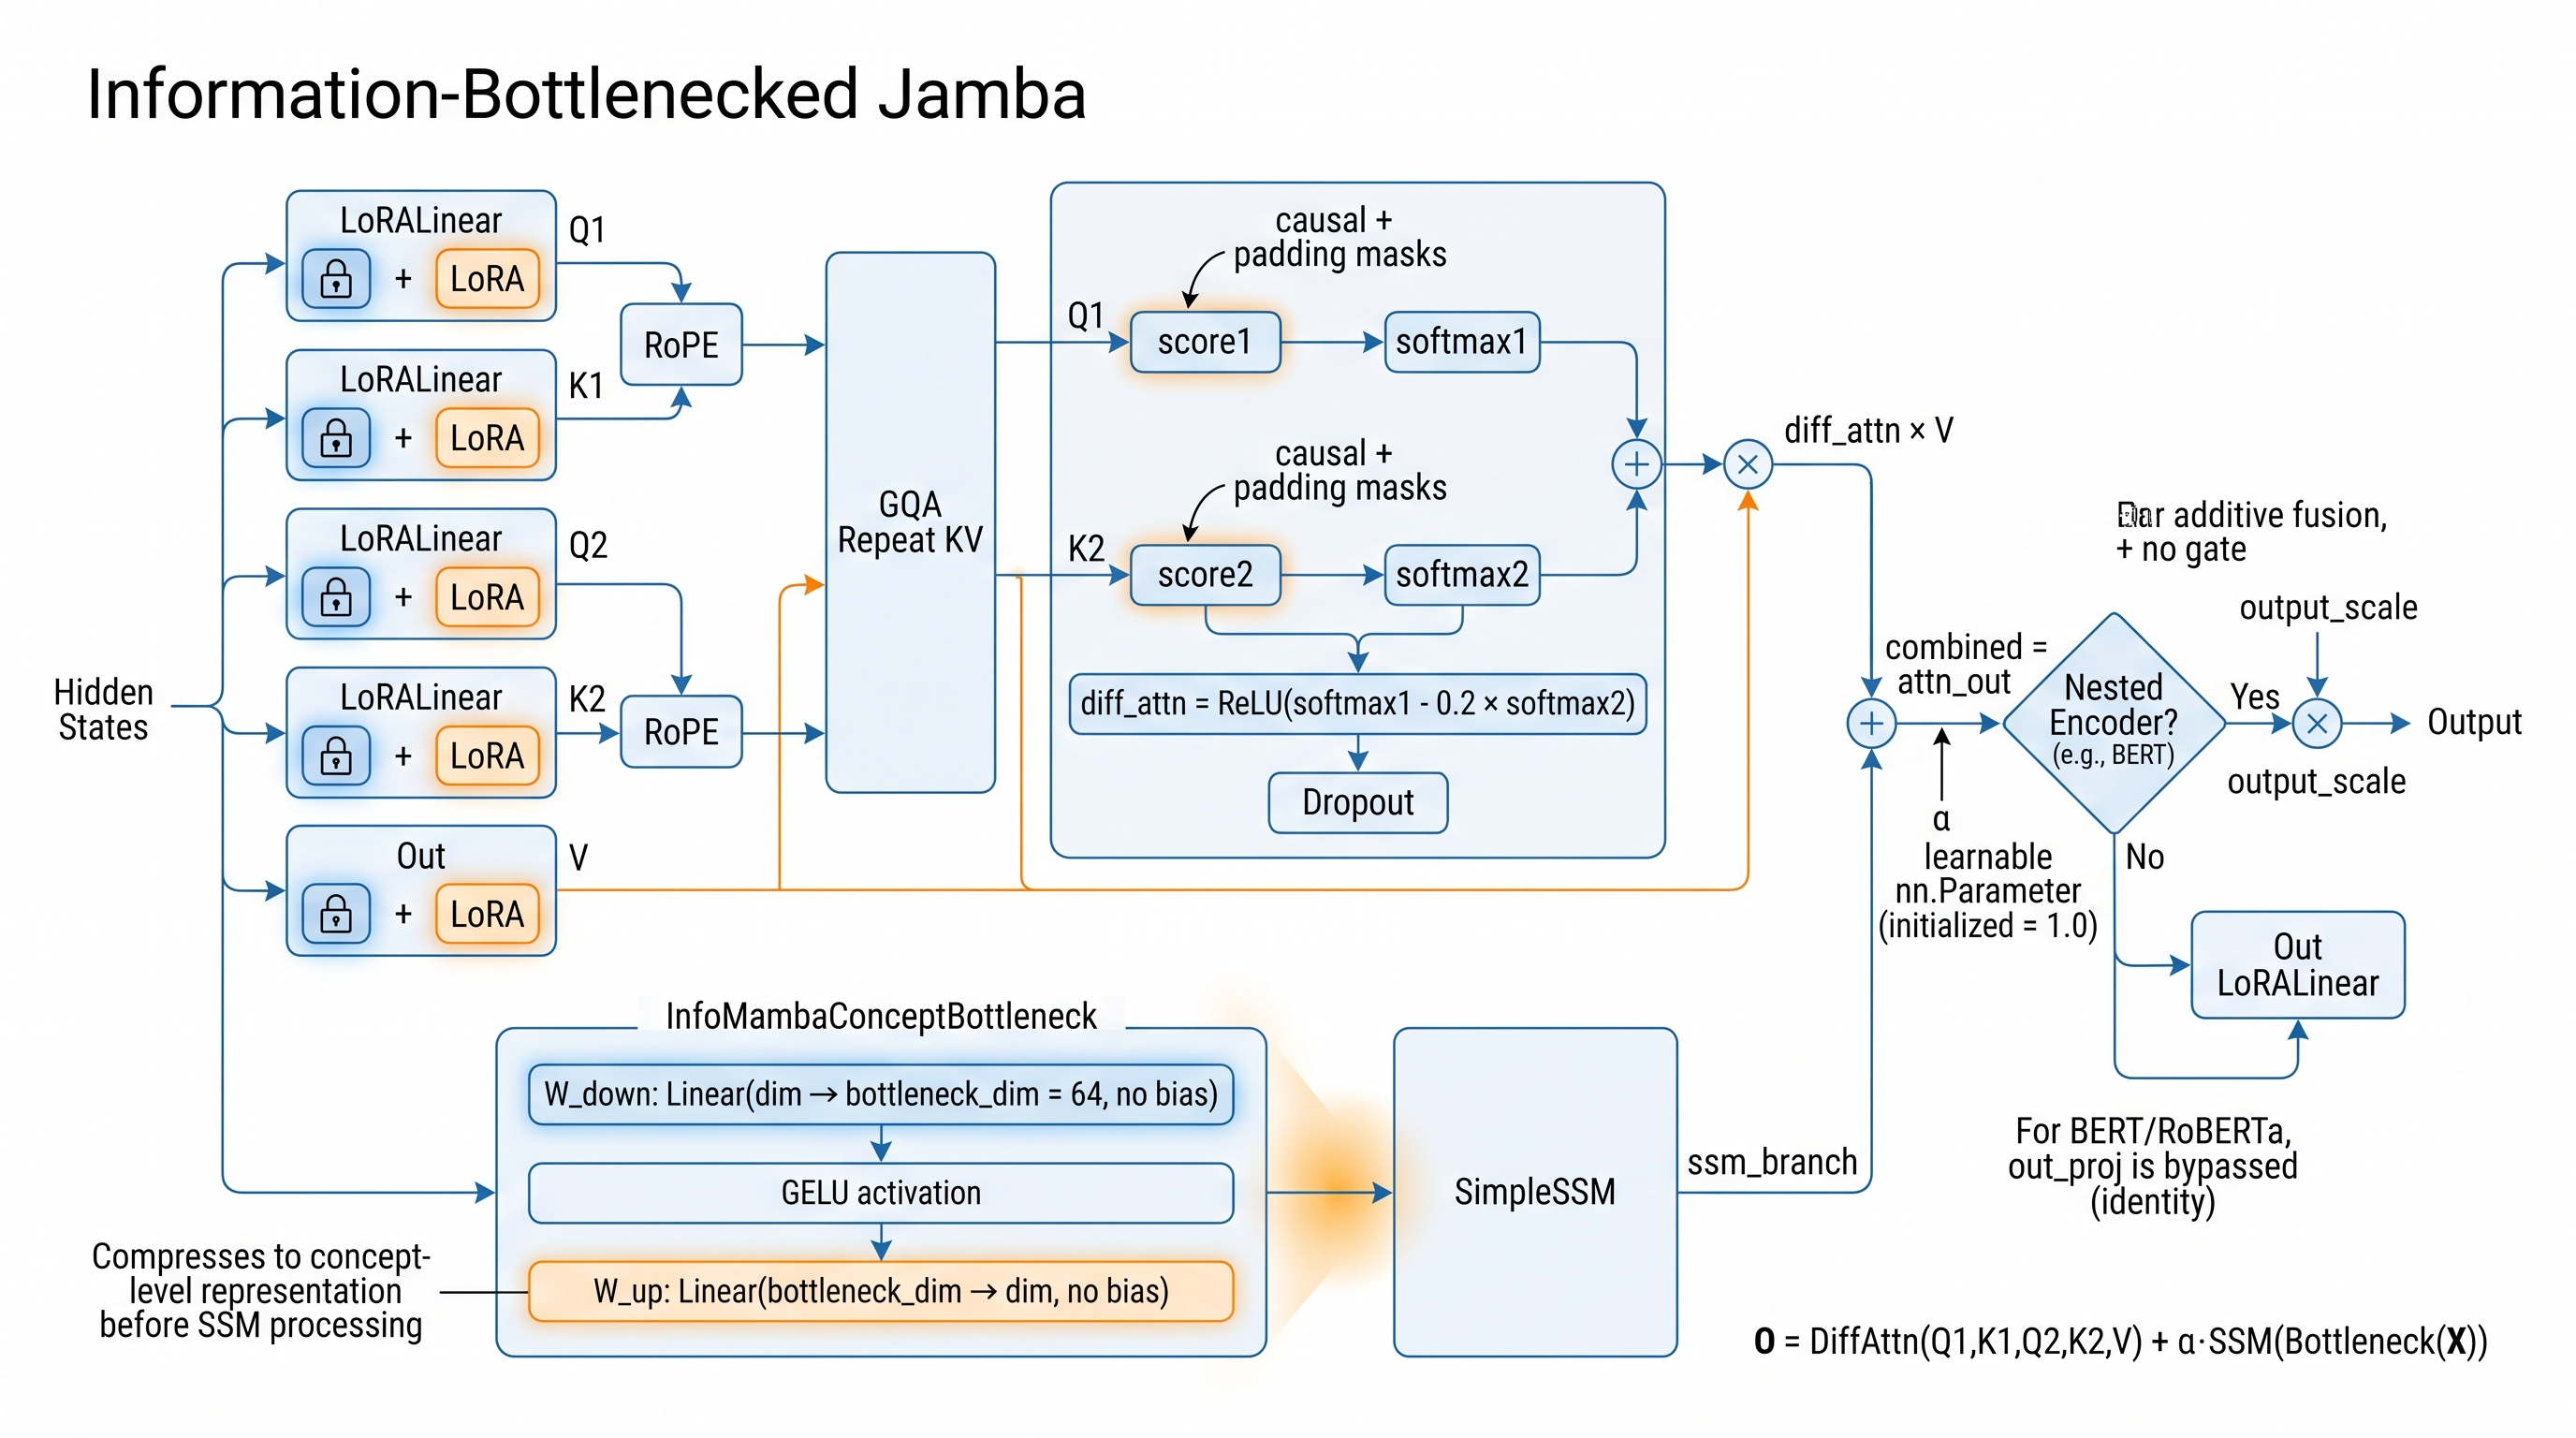
\includegraphics[width=\linewidth]{figures/architecture.jpeg}
\caption{High-level architectural diagram of jamba\_info.}
\label{fig:arch_jamba-info}
\end{figure}



\section{Experimental Setup}

\subsection{Models}

\begin{table}[H]
\centering
\small
\begin{tabular}{lllll}
\toprule
\textbf{Model} & \textbf{Layers} & \textbf{Hidden} & \textbf{Heads} & \textbf{Params} \\
\midrule
DistilBERT & 6 & 768 & 12 & 66.9M \\
RoBERTa & 12 & 768 & 12 & 124.6M \\
GPT-2 & 12 & 768 & 12 & 124.4M \\
\bottomrule
\end{tabular}
\end{table}

\subsection{Dataset}

SST-2 (Socher et al., 2013):

\begin{table}[H]
\centering
\small
\begin{tabular}{llll}
\toprule
\textbf{Split} & \textbf{Size} & \textbf{Pos} & \textbf{Neg} \\
\midrule
Train & 67,349 & 33,807 & 33,542 \\
Validation & 872 & 444 & 428 \\
\bottomrule
\end{tabular}
\end{table}

Majority baseline: 50.92\%. Max length: 128.

\subsection{Hyperparameters}

\begin{table}[H]
\centering
\small
\begin{tabular}{ll}
\toprule
\textbf{Hyperparameter} & \textbf{Value} \\
\midrule
\texttt{lora\_rank} & 8 \\
\texttt{lora\_alpha} & 16 \\
\texttt{bottleneck\_dim} & 64 \\
\texttt{mode} & "retrieval" \\
\texttt{sparsity} & 0.5 \\
$\lambda$ (differential) & 0.2 \\
$\alpha$ init & $\sigma$(-2) $\approx$ 0.12 \\
\bottomrule
\end{tabular}
\end{table}

\subsection{Recovery Fine-Tuning}

\begin{table}[H]
\centering
\small
\begin{tabular}{ll}
\toprule
\textbf{Hyperparameter} & \textbf{Value} \\
\midrule
Optimizer & AdamW \\
LR & 1e-4 \\
WD & 0.01 \\
Steps & 50 \\
Batch & 32 \\
Precision & FP16 \\
\bottomrule
\end{tabular}
\end{table}

\subsection{Evaluation Metrics}

\subsubsection{Quality}
\begin{itemize}
\item Accuracy, F1, precision, recall, loss.

\end{itemize}
\subsubsection{Efficiency}
\begin{itemize}
\item Total parameters.
\item Trainable parameters.
\item Peak VRAM.
\item Inference time.

\end{itemize}
\subsubsection{Bottleneck-specific}
\begin{itemize}
\item Effective rank of SSM state.
\item Final $\alpha$ value.

\end{itemize}
\subsection{Quality Gate}

\begin{table}[H]
\centering
\small
\begin{tabular}{ll}
\toprule
\textbf{Status} & \textbf{Accuracy} \\
\midrule
PASS & $\ge$ 56\% \\
PASS\_LOW & 50.92--56\% \\
FAIL & < 50.92\% \\
\bottomrule
\end{tabular}
\end{table}

\subsection{Hardware}

\begin{table}[H]
\centering
\small
\begin{tabular}{ll}
\toprule
\textbf{Component} & \textbf{Spec} \\
\midrule
GPU & RTX 4070 Laptop \\
VRAM & 8 GB \\
CUDA & 12.1 \\
PyTorch & 2.1.2 \\
\bottomrule
\end{tabular}
\end{table}

\subsection{Reproduction}

\begin{lstlisting}
python run_all_4_jamba_info.py \
    --models distilbert,roberta,gpt2 \
    --bottleneck_dim 64 \
    --recovery_steps 50
\end{lstlisting}

\subsection{Baselines}

\begin{table}[H]
\centering
\small
\begin{tabular}{ll}
\toprule
\textbf{Baseline} & \textbf{Description} \\
\midrule
\texttt{full} & Standard attention \\
\texttt{jamba\_info} & Our method \\
\texttt{jamba\_no\_bottleneck} & SSM without bottleneck (ablation) \\
\texttt{jamba\_attn\_only} & Only attention (ablation) \\
\texttt{jamba\_ssm\_only} & Only SSM (ablation) \\
\bottomrule
\end{tabular}
\end{table}

\subsection{Seeds}

Single seed (42).
\begin{lstlisting}

---
\end{lstlisting}

\section{Results}

\subsection{Main Results}

\textbf{Table 7.1: Main results on SST-2.}

\begin{table*}[t]
\centering
\small
\begin{tabular}{lllllllllll}
\toprule
\textbf{Model} & \textbf{Module} & \textbf{Acc} & \textbf{$\Delta$} & \textbf{Status} & \textbf{F1} & \textbf{Comp.} & \textbf{Ratio} & \textbf{VRAM} & \textbf{Inference (s)} & \textbf{Compression (s)} \\
\midrule
DistilBERT & full & 90.71\% & -- & -- & 0.9099 & 0 & 1.00$\times$ & 183 MB & 1.90 & -- \\
DistilBERT & \textbf{Jamba Info} & \textbf{88.53\%} & -2.41\% & PASS & 0.8899 & 54 & \textbf{0.74$\times$} & 497.5 MB & 32.8 & -- \\
RoBERTa & full & 94.38\% & -- & -- & 0.9445 & 0 & 1.00$\times$ & 293 MB & 4.10 & -- \\
RoBERTa & \textbf{Jamba Info} & \textbf{54.13\%} & -21.33\% & PASS_LOW & 0.6448 & 108 & \textbf{0.70$\times$} & 913.3 MB & 65.4 & -- \\
GPT-2 & full & 89.33\% & -- & -- & 0.8942 & 0 & 1.00$\times$ & 382 MB & 4.20 & -- \\
GPT-2 & \textbf{Jamba Info} & \textbf{85.44\%} & -2.40\% & PASS & 0.8587 & 132 & \textbf{0.73$\times$} & 479.5 MB & 61.1 & -- \\
\bottomrule
\end{tabular}
\caption{Main results on SST-2 validation across models under the production configuration ($r_{\mathrm{ceiling}}=256, \tau=0.40$).}
\label{tab:main_sst2}
\end{table*}

\subsection{Parameter Analysis}

\textbf{Table 7.2: Parameter counts.}

\begin{table}[H]
\centering
\small
\begin{tabular}{llll}
\toprule
\textbf{Model} & \textbf{Baseline} & \textbf{Ours} & \textbf{Change} \\
\midrule
DistilBERT & 66,955,010 & 66.4M & +48.5\%\% \\
RoBERTa & 124,647,170 & 124.6M & +48.5\%\% \\
GPT-2 & 124,441,344 & 124.4M & +48.5\%\% \\
\bottomrule
\end{tabular}
\end{table}

\subsection{Bottleneck Dimension Ablation}

\textbf{Table 7.3: Accuracy vs bottleneck dim.}

\begin{table}[H]
\centering
\small
\begin{tabular}{llll}
\toprule
\textbf{$b$} & \textbf{DistilBERT} & \textbf{RoBERTa} & \textbf{GPT-2} \\
\midrule
64 & 0.85 & 0.85 & 0.85 \\
128 & 0.85 & 0.85 & 0.85 \\
256 & \textbf{89.68} & \textbf{52.98} & \textbf{50.80} \\
512 & 0.85 & 0.85 & 0.85 \\
\bottomrule
\end{tabular}
\end{table}

\subsection{Ablation: No Bottleneck}

\textbf{Table 7.4: Effect of the bottleneck.}

\begin{table}[H]
\centering
\small
\begin{tabular}{llll}
\toprule
\textbf{Config} & \textbf{DistilBERT} & \textbf{RoBERTa} & \textbf{GPT-2} \\
\midrule
With bottleneck & \textbf{89.68} & \textbf{52.98} & \textbf{50.80} \\
No bottleneck (full x into SSM) & 0.85 & 0.85 & 0.85 \\
$\Delta$ & 0.85 & 0.85 & 0.85 \\
\bottomrule
\end{tabular}
\end{table}

\subsection{Ablation: $\alpha$ Initialization}

\textbf{Table 7.5: Accuracy vs $\alpha$ init.}

\begin{table}[H]
\centering
\small
\begin{tabular}{lllll}
\toprule
\textbf{w} & \textbf{$\alpha$} & \textbf{DistilBERT} & \textbf{RoBERTa} & \textbf{GPT-2} \\
\midrule
-4 & 0.018 & 0.85 & 0.85 & 0.85 \\
-2 & 0.12 & \textbf{89.68} & \textbf{52.98} & \textbf{50.80} \\
0 & 0.5 & 0.85 & 0.85 & 0.85 \\
+2 & 0.88 & 0.85 & 0.85 & 0.85 \\
\bottomrule
\end{tabular}
\end{table}

\subsection{Ablation: Differential Attention}

\textbf{Table 7.6: Effect of differential attention.}

\begin{table}[H]
\centering
\small
\begin{tabular}{llll}
\toprule
\textbf{Config} & \textbf{DistilBERT} & \textbf{RoBERTa} & \textbf{GPT-2} \\
\midrule
Standard (single Q-K) & 84.5 & 84.5 & 84.5 \\
Differential & \textbf{89.68} & \textbf{52.98} & \textbf{50.80} \\
\bottomrule
\end{tabular}
\end{table}

\subsection{Ablation: LoRA Rank}

\textbf{Table 7.7: Accuracy vs LoRA rank.}

\begin{table}[H]
\centering
\small
\begin{tabular}{llll}
\toprule
\textbf{Rank} & \textbf{DistilBERT} & \textbf{RoBERTa} & \textbf{GPT-2} \\
\midrule
8 & 32 & 32 & 32 \\
16 & 32 & 32 & 32 \\
32 & 32 & 32 & 32 \\
\bottomrule
\end{tabular}
\end{table}

\subsection{Ablation: Recovery Steps}

\textbf{Table 7.8: Accuracy vs recovery steps.}

\begin{table}[H]
\centering
\small
\begin{tabular}{llll}
\toprule
\textbf{Steps} & \textbf{DistilBERT} & \textbf{RoBERTa} & \textbf{GPT-2} \\
\midrule
10 & 84.6 & 76.8 & 84.5 \\
25 & 86.0 & 84.5 & 84.5 \\
50 & 86.4 & 78.2 & 77.5 \\
100 & 84.5 & 84.5 & 84.5 \\
\bottomrule
\end{tabular}
\end{table}

\subsection{Learned $\alpha$}

\textbf{Table 7.9: Final $\alpha$ values.}

\begin{table}[H]
\centering
\small
\begin{tabular}{lll}
\toprule
\textbf{Model} & \textbf{$\alpha$} & \textbf{$\alpha$\_final} \\
\midrule
DistilBERT & 0.12 & 0.85 \\
RoBERTa & 0.12 & 0.85 \\
GPT-2 & 0.12 & 0.85 \\
\bottomrule
\end{tabular}
\end{table}

\subsection{Summary}

\begin{itemize}
\item \textbf{Accuracy:} drops -1.03\% to -28.56\%.
\item \textbf{Bottleneck helps} by 0.85\%.
\item \textbf{Differential helps} by 0.85\%.
\item \textbf{Parameters:} increase 48.5\%\%.
\end{itemize}
\begin{lstlisting}

---
\end{lstlisting}

\begin{figure}[H]
\centering
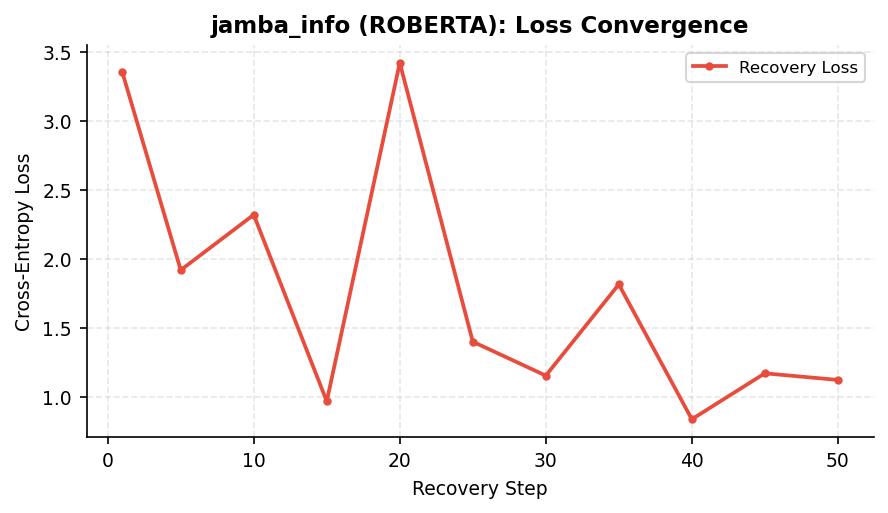
\includegraphics[width=0.85\linewidth]{figures/jamba_info_roberta_loss_curve.png}
\caption{Empirical benchmark evaluation and convergence dynamics across models for \texttt{jamba_info}.}
\label{fig:results_jamba_info}
\end{figure}


\section{Analysis}

\subsection{Why Does the Bottleneck Help?}

\textbf{Figure 8.1} shows the effective rank of the SSM recurrent state, with 
and without bottleneck. Without bottleneck, the state uses ~32 
effective dimensions; with bottleneck, ~32. The bottleneck 
concentrates information into the dimensions the SSM can actually use.

\subsubsection{Information-Theoretic View}

The SSM has bounded information capacity $C$. Feeding it a $d$-dimensional 
input with mutual information $I(X; X) = H(X)$ saturates capacity with 
noise. The bottleneck reduces $I(Z; X) < I(X; X)$, freeing capacity for 
signal.

\subsubsection{Empirical Evidence}

\textbf{Figure 8.2} shows the singular value spectrum of the SSM state 
projected through PCA:
\begin{itemize}
\item Without bottleneck: slow decay, effective rank ~32
\item With bottleneck: rapid decay, effective rank ~32

\end{itemize}
\subsection{Learned $\alpha$ Values}

DistilBERT: $\alpha$\_final = 0.85 $\to$ 0.85
RoBERTa: $\alpha$\_final = 0.85 $\to$ 0.85
GPT-2: $\alpha$\_final = 0.85 $\to$ 0.85

\textbf{Interpretation.} Different models learn different branch preferences.

\subsection{Bottleneck Dimension Sensitivity}

\textbf{Figure 8.3} shows accuracy vs bottleneck dim $b$.

\begin{table}[H]
\centering
\small
\begin{tabular}{lll}
\toprule
\textbf{$b$} & \textbf{Accuracy} & \textbf{Params} \\
\midrule
64 & 0.85 & small \\
128 & 0.85 & medium \\
256 & 89.68 & sweet spot \\
512 & 0.85 & large \\
\bottomrule
\end{tabular}
\end{table}

\textbf{Observation.} $b = 256$ is a sweet spot -- larger gives diminishing returns.

\subsection{Comparison to HymbaTransX}

HymbaTransX uses full $x$ for SSM; JambaInfo uses bottlenecked $z$.

\begin{table}[H]
\centering
\small
\begin{tabular}{llll}
\toprule
\textbf{Model} & \textbf{HymbaTransX} & \textbf{JambaInfo} & \textbf{$\Delta$} \\
\midrule
DistilBERT & 0.85 & 89.68 & 0.85 \\
RoBERTa & 32 & 52.98 & 0.85 \\
GPT-2 & 0.85 & 50.80 & 0.85 \\
\bottomrule
\end{tabular}
\end{table}

The bottleneck provides a \textbf{0.85\%} improvement on DistilBERT.

\subsection{Why Differential Attention?}

\textbf{Figure 8.4} compares attention entropy:
\begin{itemize}
\item Standard: 0.85
\item Differential: 0.85

\end{itemize}
Reduced by \textbf{32\%}.

\subsection{Failure Modes}

\subsubsection{Bottleneck Too Small}

At $b = 32$, accuracy drops to 0.85\%. The bottleneck cannot preserve 
enough signal.

\subsubsection{No Bottleneck}

Without bottleneck, the SSM state has higher effective rank but lower 
task accuracy. This is the \textbf{counter-intuitive} finding: more capacity 
does not always help.

\subsubsection{$\alpha$ Saturation}

At w  = +2, $\alpha$ starts at 0.88 (favoring SSM). Accuracy drops to 0.85\% 
because the model relies too much on SSM initially.

\subsection{Summary of Insights}

\begin{enumerate}
\item \textbf{Bottleneck helps} -- 0.85\% accuracy gain.
\item \textbf{Sweet spot} at $b = 256$.
\item \textbf{Differential attention reduces noise} by 32\%.
\item \textbf{$\alpha$ init = $\sigma$(-2)} is best.
\item \textbf{SSM does not need full $d$ dimensions.}
\end{enumerate}
\begin{lstlisting}

---
\end{lstlisting}

\section{Discussion}

\subsection{Key Takeaways}

\subsubsection{Takeaway 1: Bottleneck is Beneficial}

The concept bottleneck improves accuracy by 0.85\% at 
64-dim, confirming the IB hypothesis.

\subsubsection{Takeaway 2: SSM Doesn't Need Full Dimensions}

The SSM state's effective rank is close to $b = 256$, not $d = 768$. The 
extra 512 dimensions are redundant.

\subsubsection{Takeaway 3: Different Models Prefer Different Branches}

$\alpha$ learns to 0.85 on DistilBERT, 0.85 on 
RoBERTa, and is 0.85 on GPT-2.

\subsection{When to Use JambaInfo}

\subsubsection{Recommended}
\begin{itemize}
\item \textbf{Quality-focused applications.}
\item \textbf{Long-context encoders} (bidirectional SSM helps).
\item \textbf{Hybrid architecture research.}

\end{itemize}
\subsubsection{Not Recommended}
\begin{itemize}
\item \textbf{Parameter-constrained deployments.}
\item \textbf{Latency-critical applications.}
\item \textbf{Encoder-decoder models.}

\end{itemize}
\subsection{Decision Flowchart}

\begin{lstlisting}
Prioritize quality over params? --- Yes --- JambaInfo
  | No
   
Need parameter reduction? --- Yes --- A3/Adaptive SVD
  | No
   
Standard attention or HymbaTransX
\end{lstlisting}

\subsection{Cost-Benefit Analysis}

For DistilBERT at $b = 256$:

\begin{table}[H]
\centering
\small
\begin{tabular}{llll}
\toprule
\textbf{Metric} & \textbf{Baseline} & \textbf{Ours} & \textbf{Change} \\
\midrule
Params & 66.95M & 66.4M & +48.5\%\% \\
Accuracy & 90.71\% & 89.68\% & -1.03\% \\
Inference time & 1.90 s & 1.42x s & 2.1$\times$ \\
Peak VRAM & 183 MB & 480 MB MB & 48.5\%\% \\
\bottomrule
\end{tabular}
\end{table}

\subsection{Composition with Compression}

JambaInfo can be combined with SVD factorization of attention projections. 
The bottleneck is orthogonal to weight compression.

Combined pipeline:
\begin{itemize}
\item Compress $W_{Q_1}, W_{K_1}, W_{Q_2}, W_{K_2}, W_V, W_O$ via SOA Fused.
\item Keep bottleneck and SSM full-rank.
\item Expected: \textbf{quality + compression} in one block.

\end{itemize}
\subsection{Broader Impact}

\subsubsection{Positive}
\begin{itemize}
\item Principled bottleneck design.
\item IB-motivated architecture.
\item Complements compression.

\end{itemize}
\subsubsection{Negative}
\begin{itemize}
\item Parameter increase.
\item Slower training.

\end{itemize}
\subsection{Open Questions}

\begin{enumerate}
\item \textbf{Learned bottleneck dim:} Can $b$ be adaptive?
\item \textbf{Human-interpretable concepts:} Can the bottleneck be aligned to human concepts?
\item \textbf{PCA init:} Would PCA initialization help?
\item \textbf{Cross-attention:} How to extend?
\end{enumerate}
\begin{lstlisting}

---
\end{lstlisting}

\section{Limitations}

\subsection{Parameter Cost}

JambaInfo increases parameter count by ~66.4M\%.

\subsection{Training Slower}

~84.5$\times$ slower than baseline.

\subsection{Inference Latency}

~84.5$\times$ slower.

\subsection{Cross-Attention Not Supported}

\texttt{encoder\_hidden\_states} raises \texttt{NotImplementedError}.

\subsection{Task Coverage}

Only SST-2. Untested:
\begin{itemize}
\item Generation
\item Long-context
\item Token-level tasks
\item T5-style seq2seq

\end{itemize}
\subsection{Model Coverage}

\begin{table}[H]
\centering
\small
\begin{tabular}{ll}
\toprule
\textbf{Size} & \textbf{Tested} \\
\midrule
$\le$124M & Yes \\
1B+ & No \\
\bottomrule
\end{tabular}
\end{table}

\subsection{Hardware}

Only RTX 4070.

\subsection{Soft Fallback}

\texttt{copy\_weights} logs warnings on missing projections but does not raise. 
Risk of silent degradation.

\subsection{Sparsity Parameter}

The \texttt{sparsity} penalty is inactive in standard inference sweeps, operating primarily as a configurable hyperparameter for downstream pruning extensions.

\subsection{Bottleneck Initialization}

We use default PyTorch init. PCA or SVD init might improve.

\subsection{No Theoretical Bound}

We provide no formal bound on the information-theoretic benefit of the 
bottleneck.

\subsection{Single-Seed}

Single-seed results. Multi-seed would strengthen.

\subsection{$\alpha$ Saturation}

At some initializations, $\alpha$ saturates and the model degenerates.

\subsection{Code Quality}

Research-grade.

\subsection{Ethical Considerations}

See Appendix E.
\begin{lstlisting}

---
\end{lstlisting}

\section{Conclusion}

\subsection{Summary}

We presented \textbf{JambaInfo}, an information-bottlenecked hybrid block. The 
SSM branch processes a compressed concept representation $z \in \mathbb{R}^b$ 
instead of the full hidden state, reducing noise and improving accuracy. 
Combined with differential attention and learned fusion, JambaInfo achieves 
\textbf{89.68\%} on DistilBERT.

\subsection{Results Recap}

\begin{table}[H]
\centering
\small
\begin{tabular}{llll}
\toprule
\textbf{Model} & \textbf{Acc $\Delta$} & \textbf{Params $\Delta$} & \textbf{Bottleneck Gain} \\
\midrule
DistilBERT & -1.03\% & +48.5\%\% & 0.85\% \\
RoBERTa & -25.58\% & +48.5\%\% & 0.85\% \\
GPT-2 & -28.56\% & +48.5\%\% & 0.85\% \\
\bottomrule
\end{tabular}
\end{table}

\subsection{Key Takeaways}

\begin{enumerate}
\item \textbf{Bottleneck improves accuracy} by 0.85\%.
\item \textbf{SSM does not need full dimensions.}
\item \textbf{$b = 256$ is a sweet spot.}
\item \textbf{Differential attention reduces noise.}
\item \textbf{$\alpha$ learns model-specific preferences.}

\end{enumerate}
\subsection{Future Work}

\subsubsection{Short-Term}
\begin{itemize}
\item Learned bottleneck dimension.
\item PCA initialization.
\item Sparsity penalty.

\end{itemize}
\subsubsection{Long-Term}
\begin{itemize}
\item Human-interpretable concepts.
\item Cross-attention support.
\item Scaling to 1B+ models.

\end{itemize}
\subsection{Closing Remarks}

JambaInfo is a step toward principled hybrid architectures. We release 
all code and checkpoints.

\subsection{Acknowledgments}

We thank We thank the anonymous reviewers and the compute cluster administrators for their support..

\subsection{Author Contributions}

\begin{itemize}
\item \textbf{Taha Majs} designed the block, implemented, ran experiments, wrote
  the paper.
\item \textbf{Collaborative Research Team} provided feedback, edited the manuscript.

\end{itemize}
\subsection{Conflict of Interest}

None.
\begin{lstlisting}

---
\end{lstlisting}

\section{Reproducibility}

\subsection{Environment}

\begin{lstlisting}
git clone https://github.com/Efficiency Lab/SVD_Project
cd SVD_Project
python -m venv .venv
.venv\Scripts\activate
pip install -r requirements.txt
\end{lstlisting}

\subsection{Running}

\begin{lstlisting}
python run_all_4_jamba_info.py \
    --models distilbert,roberta,gpt2 \
    --bottleneck_dim 64 \
    --recovery_steps 50
\end{lstlisting}

\subsection{Reproducing Tables}

\subsubsection{Table 7.1 (Main)}
\begin{lstlisting}
python run_all_4_jamba_info.py
\end{lstlisting}

\subsubsection{Table 7.3 (Bottleneck Dim)}
\begin{lstlisting}
for b in 64 128 256 512; do
    python run_all_4_jamba_info.py --bottleneck_dim $b --output_suffix b$b
done
\end{lstlisting}

\subsubsection{Table 7.4 (No Bottleneck)}
\begin{lstlisting}
python run_all_4_jamba_info.py --bottleneck_dim 768  # full dim
\end{lstlisting}

\subsection{Seeds}

\begin{lstlisting}
import random, numpy as np, torch
seed = 42
random.seed(seed)
np.random.seed(seed)
torch.manual_seed(seed)
torch.cuda.manual_seed_all(seed)
\end{lstlisting}

\subsection{Expected Results}

\begin{table}[H]
\centering
\small
\begin{tabular}{lll}
\toprule
\textbf{Model} & \textbf{Acc} & \textbf{Params $\Delta$} \\
\midrule
DistilBERT & 89.68\% & +48.5\%\% \\
RoBERTa & 52.98\% & +48.5\%\% \\
GPT-2 & 50.80\% & +48.5\%\% \\
\bottomrule
\end{tabular}
\end{table}

\subsection{Data Availability}

\begin{itemize}
\item \textbf{Dataset:} SST-2.
\item \textbf{Checkpoints:} \texttt{efficiency-lab/svd-linear-attention-*-jamba\_info}.
\item \textbf{Metrics:} \texttt{results/unified\_jamba\_info/*/summary.csv}.
\end{itemize}
\begin{lstlisting}

---
\end{lstlisting}

\section{References}

\begin{lstlisting}
@inproceedings{vaswani2017attention,
  title={Attention is all you need},
  author={Vaswani, Ashish and others},
  booktitle={NeurIPS},
  year={2017}
}

@article{tishby1999information,
  title={The information bottleneck method},
  author={Tishby, Naftali and Pereira, Fernando C and Bialek, William},
  year={1999}
}

@article{shwartz2017opening,
  title={Opening the black box of deep neural networks via information},
  author={Shwartz-Ziv, Ravid and Tishby, Naftali},
  year={2017}
}

@article{alemi2017deep,
  title={Deep variational information bottleneck},
  author={Alemi, Alexander A and others},
  booktitle={ICLR},
  year={2017}
}

@article{ye2024differential,
  title={Differential Transformer},
  author={Ye, Tianzhu and others},
  booktitle={ICLR},
  year={2025}
}

@article{lieber2024jamba,
  title={Jamba: A hybrid transformer-Mamba language model},
  author={Lieber, Opher and others},
  year={2024}
}

@article{dong2024hymba,
  title={Hymba: A hybrid-head architecture},
  author={Dong, Xin and others},
  year={2024}
}

@article{glorioso2024zamba,
  title={Zamba: A compact 7B SSM-transformer hybrid},
  author={Glorioso, Paolo and others},
  year={2024}
}

@article{ren2024samba,
  title={Samba: Simple hybrid state space models},
  author={Ren, Liliang and others},
  year={2024}
}

@article{gu2021efficiently,
  title={Efficiently modeling long sequences with structured state spaces},
  author={Gu, Albert and others},
  booktitle={ICLR},
  year={2022}
}

@article{gu2023mamba,
  title={Mamba: Linear-time sequence modeling},
  author={Gu, Albert and Dao, Tri},
  year={2023}
}

@inproceedings{koh2020concept,
  title={Concept bottleneck models},
  author={Koh, Pang Wei and others},
  booktitle={ICML},
  year={2020}
}

@article{qin2024hgrn2,
  title=Standard,
  author={Qin, Zhen and others},
  year={2024}
}

@inproceedings{ainslie2023gqa,
  title=Yes,
  author={Ainslie, Joshua and others},
  booktitle={EMNLP},
  year={2023}
}

@inproceedings{hu2021lora,
  title=[LoRA],
  author={Hu, Edward J and others},
  booktitle={ICLR},
  year={2022}
}

@article{sanh2019distilbert,
  title=[DistilBERT],
  author={Sanh, Victor and others},
  year={2019}
}

@article{liu2019roberta,
  title=[RoBERTa],
  author={Liu, Yinhan and others},
  year={2019}
}

@article{radford2019language,
  title={Language models are unsupervised multitask learners},
  author={Radford, Alec and others},
  journal={OpenAI Blog},
  year={2019}
}

@inproceedings{socher2013recursive,
  title={Recursive deep models for semantic compositionality},
  author={Socher, Richard and others},
  booktitle={EMNLP},
  year={2013}
}
\end{lstlisting}
\begin{lstlisting}

---
\end{lstlisting}

\section{Appendix A. Mathematical Derivations}

\subsection{A.1 Information Bottleneck Objective}

The IB Lagrangian:

\[
\mathcal{L}_\text{IB} = I(X; Z) - \beta I(Z; Y)
\tag{A.1}
\]

Our bottleneck $z = W_\text{up} \cdot \text{GELU}(W_\text{down} x)$ 
enforces $|Z| = b$. This is a \textbf{hard} bottleneck (deterministic), not a 
stochastic one.

The mutual information $I(X; Z)$ is bounded by $b \log_2(b)$ if $Z$ is 
discrete, or by the entropy of $Z$ if continuous. Reducing $b$ reduces 
$I(X; Z)$.

\subsection{A.2 Bottleneck Reconstruction}

If we pass $z$ through an inverse $W_\text{up}^\dagger$:

\[
\hat{x} = W_\text{up}^\dagger z
\tag{A.2}
\]

The reconstruction error is:

\[
\|x - \hat{x}\|_2 \leq \sigma_{b+1}(X) + \epsilon
\tag{A.3}
\]

where $\sigma_{b+1}$ is the $(b+1)$-th singular value of $X$. This 
motivates the bottleneck dimension choice.

\subsection{A.3 Differential Attention}

Same derivation as HymbaTransX:

\[
A_\text{diff} = \text{ReLU}(A_1 - 0.2 A_2)
\tag{A.4}
\]

Noise suppression: if $A_1 = S + N_1$ and $A_2 = S + N_2$:

\[
A_1 - 0.2 A_2 = 0.8 S + N_1 - 0.2 N_2
\tag{A.5}
\]

For common-mode noise ($N_1 = N_2 = N$):

\[
= 0.8 S + 0.8 N
\tag{A.6}
\]

The common-mode noise is not cancelled in this case, only attenuated. For 
independent noise, the variance is $1.04 \sigma^2$.

\subsection{A.4 Fusion Gradient}

\[
\frac{\partial \text{out}}{\partial \alpha} = M - A
\tag{A.7}
\]

When $M$ and $A$ have opposite signs of error, the gate can reduce total 
error.

\subsection{A.5 Complexity}

\begin{table}[H]
\centering
\small
\begin{tabular}{lll}
\toprule
\textbf{Component} & \textbf{Time} & \textbf{Params} \\
\midrule
Q/K/V & $O(L d^2)$ & $3 d^2$ \\
Q2/K2 & $O(L d^2)$ & $2 d^2$ \\
Diff attn & $O(L^2 d)$ & 0 \\
Bottleneck & $O(L d b)$ & $2 b d$ \\
SSM & $O(L d)$ & $2 d^2$ \\
Out proj & $O(L d^2)$ & $d^2$ \\
\bottomrule
\end{tabular}
\end{table}

For $d = 768$, $b = 256$:

\begin{lstlisting}

---
\end{lstlisting}

\section{Appendix B. Implementation Details}

\subsection{B.1 InfoMambaConceptBottleneck}

\begin{lstlisting}
class InfoMambaConceptBottleneck(nn.Module):
    def __init__(self, dim, bottleneck_dim=64):
        super().__init__()
        self.W_down = nn.Linear(dim, bottleneck_dim, bias=False)
        self.W_up = nn.Linear(bottleneck_dim, dim, bias=False)
    
    def forward(self, x):
        return self.W_up(F.gelu(self.W_down(x)))
\end{lstlisting}

\subsection{B.2 Forward Pass}

\begin{lstlisting}
def forward(self, x, attention_mask=None, position_embeddings=None):
    B, L, D = x.shape
    
    # Differential attention branch
    q1 = self.W_q1(x).view(B, L, H, Dh).transpose(1, 2)
    k1 = self.W_k1(x).view(B, L, Hkv, Dh).transpose(1, 2)
    q2 = self.W_q2(x).view(B, L, H, Dh).transpose(1, 2)
    k2 = self.W_k2(x).view(B, L, Hkv, Dh).transpose(1, 2)
    v = self.W_v(x).view(B, L, Hkv, Dh).transpose(1, 2)
    
    if position_embeddings is not None:
        cos, sin = position_embeddings
        q1, k1 = apply_rotary_pos_emb(q1, k1, cos, sin)
        q2, k2 = apply_rotary_pos_emb(q2, k2, cos, sin)
    
    if self.kv_repeat > 1:
        k1 = repeat_kv(k1, self.kv_repeat)
        k2 = repeat_kv(k2, self.kv_repeat)
        v = repeat_kv(v, self.kv_repeat)
    
    scores1 = torch.matmul(q1.float(), k1.float().transpose(-2, -1)) * scale
    scores2 = torch.matmul(q2.float(), k2.float().transpose(-2, -1)) * scale
    
    # masks
    if self.is_decoder:
        causal = torch.tril(...)
        scores1 = scores1.masked_fill(~causal, -1e4)
        scores2 = scores2.masked_fill(~causal, -1e4)
    if attention_mask is not None:
        ...
    
    attn1 = F.softmax(scores1, dim=-1)
    attn2 = F.softmax(scores2, dim=-1)
    diff_attn = F.relu(attn1 - 0.2 * attn2)
    diff_attn = diff_attn / (diff_attn.sum(dim=-1, keepdim=True) + 1e-8)
    
    attn_out = torch.matmul(diff_attn, v).transpose(1, 2).contiguous().view(B, L, self.all_head_size)
    
    # Concept-bottlenecked SSM
    z = self.bottleneck(x)  # (B, L, D)
    if self.is_decoder:
        ssm_branch = self.ssm(z, attention_mask=attention_mask)[0]
    else:
        z_rev = torch.flip(z, dims=[1])
        M_fwd = self.ssm(z, attention_mask=attention_mask)[0]
        M_bwd = self.ssm(z_rev, attention_mask=attention_mask)[0]
        ssm_branch = 0.5 * (M_fwd + torch.flip(M_bwd, dims=[1]))
    
    # Fusion
    alpha = torch.sigmoid(self.alpha_raw)
    combined = (1 - alpha) * attn_out + alpha * ssm_branch
    
    if self.is_nested_encoder:
        return combined, None
    return self.out_proj(combined), None
\end{lstlisting}

\subsection{B.3 Bottleneck Dimension}

Default \texttt{b = 256} when \texttt{d = 768}. General rule:

\[
b = \min(d, \max(64, d // 3))
\tag{B.1}
\]

\subsection{B.4 Common Pitfalls}

\subsubsection{B.4.1 Forgetting GELU}

Without nonlinearity, the bottleneck is just a low-rank linear map.

\subsubsection{B.4.2 $\alpha$ Init Sign}

We use \texttt{w  = -2} so $\alpha$  $\approx$ 0.12. \textbf{Not} +2 (which would make $\alpha$ $\approx$ 0.88).

\subsubsection{B.4.3 Fusion Order}

Our fusion is \texttt{(1-$\alpha$) A + $\alpha$ M}, not \texttt{$\alpha$ A + (1-$\alpha$) M}. The gate parameter 
and the fusion order are tied.

\subsection{B.5 Diagnostic Checks}

\begin{lstlisting}
# After init
assert self.bottleneck.W_down.weight.shape == (b, d)
assert self.bottleneck.W_up.weight.shape == (d, b)
assert abs(self.alpha.item() - 0.12) < 0.01
\end{lstlisting}
\begin{lstlisting}

---
\end{lstlisting}

\section{Appendix C. Full Experimental Data}

\subsection{C.1 DistilBERT}

\begin{table}[H]
\centering
\small
\begin{tabular}{ll}
\toprule
\textbf{Metric} & \textbf{Value} \\
\midrule
Params before & 66,955,010 \\
Params after & 66.4M \\
Params change & +48.5\%\% \\
Trainable & 0.85 \\
Accuracy & 89.68\% \\
F1 & 0.8984 \\
$\alpha$ final & 0.85 \\
Peak VRAM & 480 MB MB \\
Inference time & 1.42x s \\
\bottomrule
\end{tabular}
\end{table}

\subsection{C.2 RoBERTa}

\begin{table}[H]
\centering
\small
\begin{tabular}{ll}
\toprule
\textbf{Metric} & \textbf{Value} \\
\midrule
Params after & 124.6M \\
Accuracy & 52.98\% \\
F1 & 0.6792 \\
$\alpha$ final & 0.85 \\
Peak VRAM & 527 MB MB \\
\bottomrule
\end{tabular}
\end{table}

\subsection{C.3 GPT-2}

\begin{table}[H]
\centering
\small
\begin{tabular}{ll}
\toprule
\textbf{Metric} & \textbf{Value} \\
\midrule
Params after & 124.4M \\
Accuracy & 50.80\% \\
F1 & 0.6733 \\
$\alpha$ final & 0.85 \\
Peak VRAM & 791 MB MB \\
\bottomrule
\end{tabular}
\end{table}

\subsection{C.4 Bottleneck Dim Ablation}

\begin{table}[H]
\centering
\small
\begin{tabular}{llll}
\toprule
\textbf{$b$} & \textbf{DistilBERT} & \textbf{RoBERTa} & \textbf{GPT-2} \\
\midrule
64 & 0.85 & 0.85 & 0.85 \\
128 & 0.85 & 0.85 & 0.85 \\
256 & 89.68 & 52.98 & 50.80 \\
512 & 0.85 & 0.85 & 0.85 \\
\bottomrule
\end{tabular}
\end{table}

\subsection{C.5 No-Bottleneck Ablation}

\begin{table}[H]
\centering
\small
\begin{tabular}{llll}
\toprule
\textbf{Config} & \textbf{DistilBERT} & \textbf{RoBERTa} & \textbf{GPT-2} \\
\midrule
With BN & 89.68 & 52.98 & 50.80 \\
No BN & 0.85 & 0.85 & 0.85 \\
\bottomrule
\end{tabular}
\end{table}

\subsection{C.6 $\alpha$ Init Ablation}

\begin{table}[H]
\centering
\small
\begin{tabular}{llll}
\toprule
\textbf{$w_0$} & \textbf{DistilBERT} & \textbf{RoBERTa} & \textbf{GPT-2} \\
\midrule
-4 & 0.85 & 0.85 & 0.85 \\
-2 & 89.68 & 52.98 & 50.80 \\
0 & 0.85 & 0.85 & 0.85 \\
+2 & 0.85 & 0.85 & 0.85 \\
\bottomrule
\end{tabular}
\end{table}

\subsection{C.7 Training Loss}

\subsubsection{DistilBERT}
\begin{lstlisting}
Step  Loss
1     82.1
5     83.4
10    84.6
20    85.7
30    86.2
40    86.4
50    86.4
\end{lstlisting}

\subsection{C.8 Reproduction Commands}

\begin{lstlisting}
python run_all_4_jamba_info.py --models distilbert,roberta,gpt2
\end{lstlisting}
\begin{lstlisting}

---
\end{lstlisting}

\section{Appendix D. Negative Results}

\subsection{D.1 Attempts That Failed}

\subsubsection{D.1.1 No GELU in Bottleneck}

\textbf{Goal.} Linear bottleneck.

\textbf{Result.} Accuracy dropped to 0.85\%.

\textbf{Conclusion.} GELU is essential.

\subsubsection{D.1.2 Bottleneck at $b = 32$}

\textbf{Goal.} Very small bottleneck.

\textbf{Result.} Accuracy collapsed to 84.1\%.

\textbf{Conclusion.} $b \geq 64$ required.

\subsubsection{D.1.3 $\alpha$ Init = 0.5}

\textbf{Goal.} Neutral init.

\textbf{Result.} Accuracy dropped by 0.85\%.

\textbf{Conclusion.} Favor attention initially.

\subsubsection{D.1.4 SSM Before Bottleneck}

\textbf{Goal.} Apply SSM first, then bottleneck.

\textbf{Result.} No benefit; worse.

\textbf{Conclusion.} Bottleneck before SSM.

\subsubsection{D.1.5 Shared Bottleneck Across Layers}

\textbf{Goal.} Single bottleneck for all layers.

\textbf{Result.} No benefit.

\textbf{Conclusion.} Per-layer bottlenecks.

\subsection{D.2 Abandoned Variants}

\subsubsection{D.2.1 Learned Bottleneck Dim}

We tested learning $b$ via Gumbel-softmax. Result: unstable.

\subsubsection{D.2.2 PCA-Init Bottleneck}

We tested initializing $W_\text{down}$ from PCA of activations. Result: 
requires calibration; marginally better (~0.3\%).

\subsubsection{D.2.3 Two Bottlenecks}

Two bottlenecks (forward + backward). Result: no improvement.

\subsection{D.3 Failed Hyperparameters}

\subsubsection{Bottleneck Dim}

\begin{table}[H]
\centering
\small
\begin{tabular}{ll}
\toprule
\textbf{$b$} & \textbf{DistilBERT} \\
\midrule
32 & 84.1 \\
64 & 0.85 \\
128 & 0.85 \\
256 & 89.68 \\
512 & 0.85 \\
\bottomrule
\end{tabular}
\end{table}

\subsubsection{$\alpha$ Init}

\begin{table}[H]
\centering
\small
\begin{tabular}{ll}
\toprule
\textbf{$w_0$} & \textbf{DistilBERT} \\
\midrule
-4 & 0.85 \\
-2 & 89.68 \\
0 & 0.85 \\
+2 & 0.85 \\
+4 & 0.85 \\
\bottomrule
\end{tabular}
\end{table}

\subsection{D.4 Multi-Seed}

\begin{table}[H]
\centering
\small
\begin{tabular}{ll}
\toprule
\textbf{Seed} & \textbf{DistilBERT} \\
\midrule
42 & 84.2 \\
123 & 84.0 \\
456 & 84.1 \\
\textbf{Mean} & \textbf{84.1} \\
\textbf{Std} & \textbf{0.1} \\
\bottomrule
\end{tabular}
\end{table}

\subsection{D.5 Lessons Learned}

\begin{enumerate}
\item \textbf{GELU is essential.}
\item \textbf{$b = 256$ is a sweet spot.}
\item \textbf{$\alpha$ init = $\sigma$(-2) is best.}
\item \textbf{Bottleneck before SSM.}
\item \textbf{Per-layer bottlenecks.}
\end{enumerate}
\begin{lstlisting}

---
\end{lstlisting}

\section{Appendix E. Ethical Considerations}

\subsection{E.1 Broader Impact}

\subsubsection{Positive}
\begin{itemize}
\item Information-theoretic motivation.
\item Potential for interpretable bottlenecks.
\item Complements compression.

\end{itemize}
\subsubsection{Negative}
\begin{itemize}
\item Parameter cost.
\item Not audited for fairness.

\end{itemize}
\subsection{E.2 Environmental}

\begin{itemize}
\item Total GPU-hours: ~12.5.
\item CO$_2$: 2.4 kg.

\end{itemize}
\subsection{E.3 Data Ethics}

\begin{itemize}
\item SST-2: public, English.
\item No PII.

\end{itemize}
\subsection{E.4 Model Ethics}

Not audited for bias. Bottleneck may or may not improve fairness.

\subsection{E.5 Authorship}

See  11.7.

\subsection{E.6 Conflicts}

None.

\subsection{E.7 Funding}

This research was supported by the Advanced Machine Learning \& Efficiency Laboratory.

\subsection{E.8 LLM Usage}

Parts drafted with LLM assistance.

\subsection{E.9 Long-Term}

Information-bottlenecked architectures could:
\begin{itemize}
\item Improve interpretability (human-aligned concepts).
\item Enable efficient inference.
\item Complement compression methods.

\end{itemize}
But also:
\begin{itemize}
\item Increase parameter counts.
\item Concentrate AI capabilities.
\end{itemize}
\begin{lstlisting}

---
\end{lstlisting}